% ****** Start of file apssamp.tex ******
%
%   This file is part of the APS files in the REVTeX 4.2 distribution.
%   Version 4.2a of REVTeX, December 2014
%
%   Copyright (c) 2014 The American Physical Society.
%
%   See the REVTeX 4 README file for restrictions and more information.
%
% TeX'ing this file requires that you have AMS-LaTeX 2.0 installed
% as well as the rest of the prerequisites for REVTeX 4.2
%
% See the REVTeX 4 README file
% It also requires running BibTeX. The commands are as follows:
%
%  1)  latex apssamp.tex
%  2)  bibtex apssamp
%  3)  latex apssamp.tex
%  4)  latex apssamp.tex
%
\documentclass[%
 reprint,
%superscriptaddress,
%groupedaddress,
%unsortedaddress,
%runinaddress,
%frontmatterverbose, 
%preprint,
%preprintnumbers,
%nofootinbib,
%nobibnotes,
%bibnotes,
 amsmath,amssymb,
 aps,
%pra,
%prb,
%rmp,
%prstab,
%prstper,
%floatfix,
]{revtex4-2}
\usepackage{kotex}
\usepackage{graphicx}% Include figure files
\usepackage{dcolumn}% Align table columns on decimal point
\usepackage{bm}% bold math
%\usepackage{hyperref}% add hypertext capabilities
%\usepackage[mathlines]{lineno}% Enable numbering of text and display math
%\linenumbers\relax % Commence numbering lines

%\usepackage[showframe,%Uncomment any one of the following lines to test 
%%scale=0.7, marginratio={1:1, 2:3}, ignoreall,% default settings
%%text={7in,10in},centering,
%%margin=1.5in,
%%total={6.5in,8.75in}, top=1.2in, left=0.9in, includefoot,
%%height=10in,a5paper,hmargin={3cm,0.8in},
%]{geometry}

\def\rcurs{{\mbox{$\resizebox{.16in}{.08in}{
\includegraphics{ScriptR}}$}}}
\def\brcurs{{\mbox{$\resizebox{.16in}{.08in}{
\includegraphics{BoldR}}$}}}
\def\hrcurs{{\mbox{$\hat \brcurs$}}}

\begin{document}


\title{화학전지 실험 결과보고서}

\author{서울대학교 전기정보공학부 2018-12432 박정현}
 \email{alexist@snu.ac.kr}
\date{\today}% It is always \today, today,
             %  but any date may be explicitly specified

\begin{abstract}
본 실험에서는 여러 물질의 전기전도도를 확인하여 전류에 대한 이해도를 높인다. 또한 여러 금속들의 반응성을 비교해 전기화학적 서열을 실험적으로 확인하였다. 또한 아연, 구리 등과 같은 금속돌의 다니엘 전지를 만들고 전압을  측정해 네른스트식을 이해하고 검증하였다. 실험에서 나타난 대부분의 오차는 금속산화물에 의한 것으로 결론지었으며 해당 산화물을 완전히 제거하면 더 높은 정확도의 실험 결과를 얻을 것으로 결론지었다.
\end{abstract}

%\keywords{Suggested keywords}%Use showkeys class option if keyword
                              %display desired
\maketitle

%\tableofcontents

\section{\label{sec:level1}Assignment}
\subsection{\label{sec:level2}Problem1}
$298K$에서 아래와 같은 화학전지가 주어졌을 때 알짜 화학반응식은 아래와 같다.
\begin{align}
	Co(s) | Co^{2+} (0.002M) &|| Ni^{2+} (0.020M) | Ni(s)
\end{align}
\begin{align}
	Co^{2+}(aq) + 2e^{-} \rightarrow Co(s)   &E^{o} = -0.28V\\
	Ni(s) \rightarrow Ni^{2+}(aq) + 2e^{-}    &E^{o} = +0.31V\\
	 \cline{1-2}
	Co^{2+}(aq) + Ni(s) \rightarrow Co(s) + Ni^{2+}(aq) &E^{o} = +0.03V\\
	(E^{o} = +0.31 + (-0.28)V)
\end{align}

네른스트식을 이용했을 때 화학 전지의 전압은 아래와 같다.
\begin{align}
	Co^{2+}(aq) &+ Ni(s) \rightarrow Co(s) + Ni^{2+}(aq) E^{o} = 0.03V\\
	E_{cell} &=  E^{o} - \frac{0.05916}{2}\log \left( \frac{[Ni^{2+}]}{[Co^{2+}]}\right)\\
	&= 0.03 - \frac{0.05916}{2}\log\frac{0.02M}{0.002M} [V]\\
	&= 0.00042 V \times \frac{1000mV}{1V}\\
	&= 0.42mV
\end{align}
따라서 화학전지의 전압은 $E_{cell}=+0.42mV$이다.


\subsection{\label{sec:level2}Problem1}
아연의 전자배치는 $[Ar]3d^{10}4s^{2}$, 구리의 전바대치는 $[Ar]3d^{10}4s^{1}$이므로 아연이 2개의 전자를 잃게 되면 $[Ar]3d^{10}$으로 더 안정된 전자배치를 가지게 된다. 따라서 $Zn(s) \rightarrow Zn^{2+}(aq) + 2e^{-}$은 $E^{o} = -(-0.76)V = +0.76V$으로 전자를 잃는 것이 음의 깁스에너지를 가지는 것이 정반응이 되게 된다. 반면에 구리의 경우 $Cu^{2+}$의 전자배치는 $[Ar]3d^{9}$이 되어 $[Ar]3d^{10}$의 전자배치보다 안정하지 않아 $Cu(s) \rightarrow Cu^{2+}(aq) + 2e^{-}$은 $E^{o} = -(+0.34)V = -0.34V$로 양의 깁스에너지를 가져 반응이 자발적으로 일어나지 않는다. 결론적으로 전자배치의 차이에 의해 표준환원전위의 역전이 발생한다.

\section{\label{sec:level1}Data and Results}
\subsection{\label{sec:level2}전기전도성}
각각의 상황에서 측정된 전기전도성은 Tab.\ref{tab:elecond}와 같다. 이 때 전기전도성은 연결된 LED가 켜지는지의 여부에 따라 결정하였다.
\begin{table}[]
\begin{tabular}{c|c|c} \hline \hline
 물질의 종류 & 증류수 \\ \hline
전기전도성 & 흐르지 않음\\ \hline \hline
 물질의 종류 & 소금($NaCl(s)$) & 소금($NaCl(aq)$) \\ \hline
전기전도성 & 흐르지 않음 & 매우 잘 흐름 \\ \hline \hline
 물질의 종류 & 설탕($C_{12}H_{22}O_{11}(s)$) & 설탕($C_{12}H_{22}O_{11}(aq)$)\\ \hline
전기전도성 & 흐르지 않음 & 매우 미미하게 흐름 \\ \hline \hline 
\end{tabular}
\caption{\label{tab:elecond}측정된 전기전도도}
\end{table}

\subsection{\label{sec:level2}전기화학적 서열}
수용액의 종류와 금속의 종류에 따른 화학 반응 여부는 아래 Tab.\ref{tab:chemreaction}와 같다. 이 때, O는 화학반응이 일어난 경우, X는 반응이 일어나지 않은 경우를 뜻한다. 실제 반응 결과는 아래 Fig.\ref{fig:ChemREAC}과 같다.
\begin{table}[]
\begin{tabular}{c|c|c|c} \hline \hline
 & $Cu(NO_{3})_{2}$ & $Pb(NO_{3})_{2}$ & $Zn(NO_{3})_{2}$ \\ \hline
$Cu$ & - & X & X\\ \hline
$Pb$ & O & - & X\\ \hline
$Zn$ & O & O & - \\  \hline \hline 
\end{tabular}
\caption{\label{tab:chemreaction}측정된 화학 반응여부}
\end{table}

\begin{figure}[htbp]
	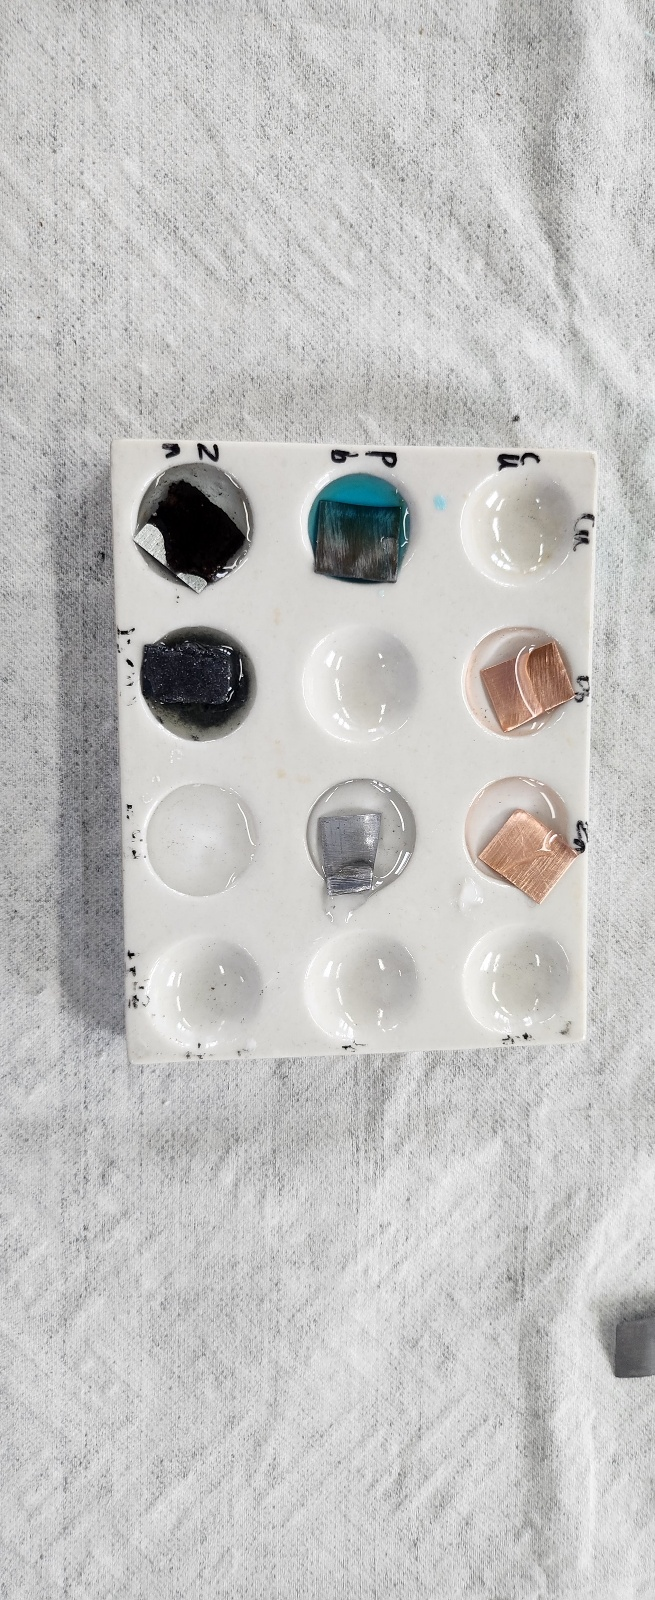
\includegraphics[angle=90, width = 0.95\linewidth]{ChemREAC.png}% Here is how to import EPS art
	\caption{\label{fig:ChemREAC}화학 반응 결과}
\end{figure}

\subsection{\label{sec:level2}화학전지 실험}
다니엘 전지에서 각 전지의 종류에 따른 측정된 전압은 Tab.\ref{tab:chemvol}와 같다. 단, 여기서 $0.001M Cu$ 와 $0.1M Zn$ 의 경우 $1.029V$에서 $0.995V$으로 값이 변화하는데 이는 시간에 따라 전압이 감소한 것을 기록한 것이다. 또한 오차는 멀티미터의 resolution에 의한 오차이다. 또한 몰농도의 오차는 모두 $1\%$이하임을 가정하였다.
\begin{table}[]
\begin{tabular}{c|c|c|c} \hline \hline
 Cathode & Anode & Measured Voltage[V] & Ideal Votalge[V] \\ \hline
$1.0M Cu$ & $1.0M Zn$ & $1.104\pm0.001$ & 1.100 \\ \hline
$1.0M Cu$ & $1.0M Pb$ & $0.614\pm0.001$ & 0.637 \\  \hline
$1.0M Zn$ & $1.0M Pb$ & $0.468\pm0.001$ & 0.463 \\ \hline
$0.1M Cu$ & $0.1M Zn$ & $1.095\pm0.001$ & 1.100 \\ \hline
$0.01M Cu$ & $0.1M Zn$ & $1.070\pm0.001$ & 1.070 \\ \hline
$0.001M Cu$ & $0.1M Zn$ & $1.029 \rightarrow 0.995\pm0.001$ & 1.041 \\ \hline
$0.1M Cu$ & $0.01M Cu$ & $0.013\pm0.001$ & 0.030\\ \hline
$0.01M Cu$ & $0.001M Cu$ & $0.013\pm0.001$ & 0.030 \\ \hline
$0.1M Cu$ & $0.001M Cu$ & $0.045\pm0.001$ & 0.059 \\ \hline \hline 
\end{tabular}
\caption{\label{tab:chemvol}측정된 전압}
\end{table}

\section{\label{sec:level1}Discussion}
\subsection{\label{sec:level2}전기전도성}
증류수의 경우 순수한 $H_{2}O$로 구성되어 있다. 따라서 $[H^{+}][OH^{-}] = 10^{-14} M^{2}$임을 이용해 중성 전하를 띠고 있는 물은 $[H^{+}] = 10^{-7}M$이므로 전류가 거의 흐르지 않을 것을 예측할 수 있으며 실제로도 전류가 흐르지 않음을 확인하였다. $NaCl(s)$의 경우 고체 상태에서는 금속의 자유전자와 같이 자유롭게 이동이 가능한 전하가 존재하지 않으므로 실험 결과와 같이 전류가 흐르지 않는다. 하지만 수용액 상태가 되는 경우 $Na^{+}(aq)$와 $Cl^{-}(aq)$로 분리되어 자유롭게 이동이 가능한 전하가 만들어지므로 측정된 실험 결과와 같이 전류가 흐르게 된다. \\


설탕의 경우 분자식을 $C_{12}H_{22}O_{11}$으로 가정했을 때 고체 상태일 경우 자유롭게 이동가능한 전하가 존재하지 않아 실험 결과와 같이 전류가 흐르지 않는다. 수용액이 되는 경우에도 대부분 중성 상태의 분자들이 수화되어 자유롭게 이동가능해지며 이 때 탄소, 수소, 산소 사이에 존재하는 전자친화도 차이로 인해 미세한 극성이 생기고 약간의 전하를 띤 분자들이 자유롭게 이동하므로 실험 결과와 같이 미미한 전류가 흐르게 된다. C의 경우 2.55, H의 경우 2.20, O의 3.44이다.[2]  모든 화학 결합은 공유결합의 성질, 그리고 이온 결합의 성질을 띠고 있는데 공유결합에서 이온화 정도를 $\exp\left(-\frac{1}{4}|X_{1}-X_{2}|^{2}\right)$을 통해 계산 가능하다. 이 때 $X_{1}$, $X_{2}$각각은 원자 $1,2$의 전기음성도이다. 가장 큰차이를 가지는 수소와 산소 사이의 이온화 정도를 계산하면 $1-\exp\left(-\frac{1}{4}|3.44-2.20|^{2}\right) = 0.31$로 약 $30\%$의 이온성을 띠고 있어 앞서 논의한 부분과 실험 결과와 일치한다. 따라서 이온 결합은 공유결합에서 전기음성도 차이가 매우 커지는 극단적인 경우로 고려할 수 있으며 이온 결합에서 발생하는 전기전도성이 공유결합에서 나타나는 이유 또한 이러한 이온 결합 성질이 공유결합에서도 나타나기 때문이라고 결론지을 수 있다. 

\subsection{\label{sec:level2}전기화학적 서열}
$Cu, Pb, Zn$ 각각의 표준 환원 전위는 아래와 같이 알려져 있다.[1] 아래 표에서 알 수 있듯 전기 화학적 서열은 $Cu > Pb > Zn$이며 실험 결과 또한 $(Pb,Cu(NO_{3})_{2}), (Zn, Pb(NO_{3})_{2}), (Zn,Cu(NO_{3})_{2})$의 쌍만 반응한 것을 통해 이론적인 예측과 일치함을 알 수 있다. 각각의 화학반응은 아래와 같다.
\begin{table}[]
\begin{tabular}{c|c|c|c} \hline \hline
 금속 & $Cu$ & $Pb$ & $Zn$ \\ \hline
표준 환원 전위$[V]$ & $ -0.763$ & $-0.126$ & $+0.337$ \\  \hline \hline 
\end{tabular}
\caption{\label{tab:STDV}표준 환원 전위}
\end{table}

\begin{align}
Pb(s)+Cu(NO_{3})_{2}(aq)\leftrightarrow Cu(s) + Pb(NO_{3})_{2}(aq)\\
Zn(s)+Cu(NO_{3})_{2}(aq)\leftrightarrow Cu(s) + Zn(NO_{3})_{2}(aq)\\
Zn(s)+Pb(NO_{3})_{2}(aq)\leftrightarrow Pb(s) + Zn(NO_{3})_{2}(aq)
\end{align}

\subsection{\label{sec:level2}화학전지 실험}
$Cu$만을 전지판으로 연결한 결과를 제외 하고 모든 결과가 네른스트 식으로 계산된 전압값과 $5\%$이내에서 일치한다. $Cu$의 경우 이론값과 차이를 보이는데 이는 $Cu$ 전지판에 형성되어 있는 산화물 $CuO$가 완전히 제거되지 않아 발생한 것으로 결론지었다. $Cu$전지판만을 이용한 경우 시간에 따른 전압 변화가 크게 나타나지 않았기 때문에 화학전지 반응에 따라 변화하는 $[Cu^{2+}]$농도 변화에 의한 효과는 무시 가능하다고 결론지었다. 화학전지 반응에 참가하는 $Cu$, $CuO$ 각각의 몰비율을 $x$, $1-x$라고 가정하는 경우 화학전지의 전압값은 근사적으로 아래와 같을 것이다. 각각의 화학반응에서 비슷한 몰 비율의 $CuO$가 화학전지 반응에 참여한 경우 constant한 효과를 줄것이다. 측정된 $Cu$ 화학전지 실험 결과 값에 $CuO$에 의한 효과를 $0.015V$으로 가정한 뒤 해당값을 모두 더해주는 경우 $0.028V$, $0.028V$, $0.060V$으로 오차가 크게 줄어들게 된다.
\begin{align}
	E^{cell} &\simeq xE^{o}_{Cu} + (1-x)E^{o}_{CuO} - \frac{0.05916}{2}\log Q
\end{align}
\\

$Cu$, $Zn$ 화학 전지에 대해서 반응비 $Q$에 대한 화학전지 전압 그래프는 Fig.\ref{fig:CuZnReac}와 같다.

\begin{figure}[htbp]
	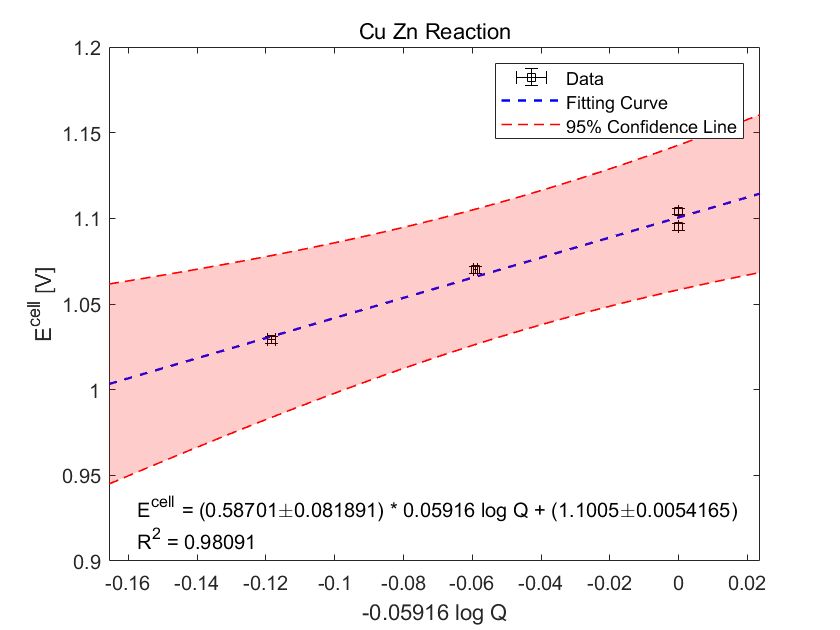
\includegraphics[width = 0.95\linewidth]{CuZnReac.png}% Here is how to import EPS art
	\caption{\label{fig:CuZnReac}$Cu$, $Zn$ 화학전지 전압}
\end{figure}

해당 그래프를 통해 측정된 반응에 참여하는 전자 수와 $E^{o}_{cell}$는 아래와 같다. $R^{2}$값이 충분히 1에 가깝고 측정된 $E^{o}_{cell}$또한 이론적으로 예측한 값에 매우 가까워 정확도와 재현도가 높게 측정되었다. $n$의 경우 이상적인 수치와 $15\%$정도의 차이가 발생한다. 이는 모든 화학전지 반응이 $Cu^{2+}(aq) +Zn(s) \rightarrow Cu(s) + Zn^{2+}(aq)$가 아니고 $Cu^{1+}(aq) +Zn(s) \rightarrow Cu(s) + Zn^{1+}(aq)$ 등과 같은 반응이 화학전지에서 나타남을 시사한다. 이외에도 온도, 그리고 $Cu$, $Zn$의 산화물에 의한 효과또한 존재한다. 하지만 충분히 $2$에 가까우므로 주요 화학전지 반응에는 전자 2개가 관여함을 알 수 있다.
\begin{align}
	n &= 1.70 \pm 0.24\\
	E^{o}_{cell} &= 1.10 \pm 0.01
\end{align}
\\

$Cu$, $Cu$ 화학 전지에 대해서 반응비 $Q$에 대한 화학전지 전압 그래프는 Fig.\ref{fig:CuCuReac}와 같다.

\begin{figure}[htbp]
	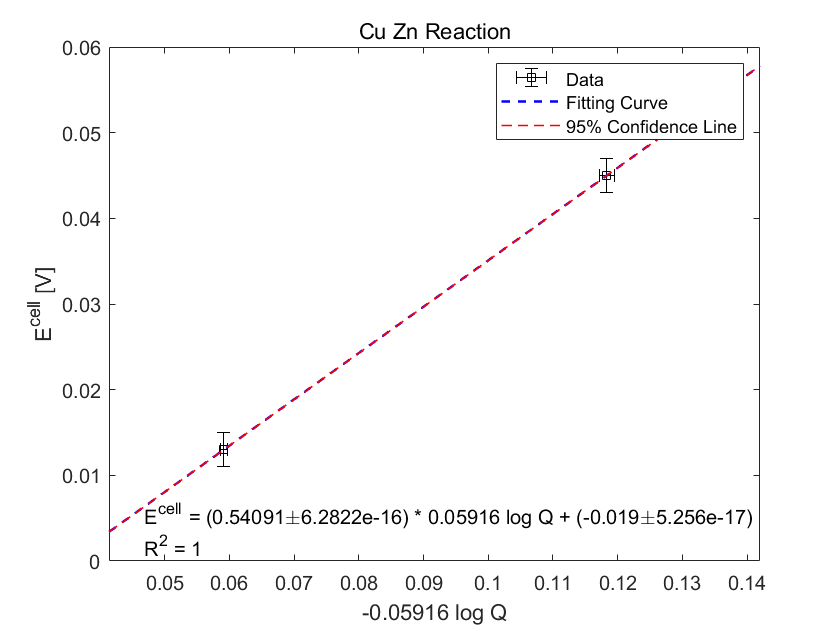
\includegraphics[width = 0.95\linewidth]{CuCuReac.png}% Here is how to import EPS art
	\caption{\label{fig:CuCuReac}$Cu$, $Cu$ 화학전지 전압}
\end{figure}

해당 그래프를 통해 측정된 반응에 참여하는 전자 수와 $E^{o}_{cell}$는 아래와 같다. $R^{2}=1$이지만 측정 데이터 수가 적어 유의미한 결과를 나타내지는 않는다. $E^{o}_{cell}$은 이론적인 예측 값 $0$에 매우 가깝다. 또한 $n$의 값 또한 이론적인 예측값 $2$에 매우 가깝다. 오차는 앞서 언급한 구리 산화물이 산화, 환원됨에 나타나는 것으로 결론지었다.
\begin{align}
	n &= 1.85 \pm 0.00\\
	E^{o}_{cell} &= -0.02 \pm 0.00
\end{align}

\section{\label{sec:level1}Conclusion}
각 물질에 따른 전기전도성은 이론적으로 예측한 바와 일치하였다. 특히 설탕에서의 약한 전기전도성을 확인하여 화학결합은 이온결합과 공유결합이 함께 공존하는 것으로 결론지었다. 설탕 뿐만 아니라 수소 결합을 하는 알코올, 페놀 등과 같은 물질의 전기전도성을 확인하여 수소 결합에 의한 전기전도도를 확인하는 실험 또한 가능할 것이다.\\

각 금속들의 전기화학적 서열은 이론적인 예측과 일치하였으나 $Pb$와 $Cu(NO_{3})_{2}$의 경우 반응이 미미하게 나타났다. 촉매를 활용해 더 확실한 실험 결과를 확인할 수 있을 것으로 기대한다.\\

각 금속으로 구성된 화학전지의 전위를 측정하였으며 이론적 예측 값과 일치함을 확인하였다. 금속 산화물을 더 완전히 제거하는 경우 실험의 정확도가 높아질 것으로 기대한다.

\section{\label{sec:level1}Reference}
[1] 김희준, \textit{일반화학 실험}(자유아카데미, 2016)\\

[2] D.W. Oxtoby, H.P. Gillis, and L. Butler, \textit{Principles of Modern Chemistry} (Brooks/Cole, Australia, 2020).

\end{document}
%
% ****** End of file apssamp.tex ******
